\section{Artifact identity and implementation trace}
\label{app:identity}
The source archive supplied for this draft is named \code{18-s44-rasch-caimira(1).zip}. Its ordinary SHA-256 is
\begin{center}\small\ttfamily
23546eb90c7469fe7ea2704879775885f1b32e3277b4b7b3a1015aa1c7c6297b
\end{center}
The filename suffix is local to the attachment. The archived submission ledger lists the same checksum and byte count under \code{18-s44-rasch-caimira.zip}, linking it to submission 1033935. Its recorded creation time is November 4, 2026, at 23:38:06 UTC, which corresponds to 15:38:06 Pacific Standard Time and agrees with the supplied screenshot's displayed minute.

\begin{table}[H]
\centering
\caption{Files inside the exact candidate archive.}
\begin{tabularx}{\linewidth}{@{}p{.45\linewidth}r>{\raggedright\arraybackslash}X@{}}
\toprule
File & Uncompressed bytes & Role \\
\midrule
\code{model.py} & 53,370 & Exported predictor and branch implementations \\
\code{caimira-requires-state.json} & 70,999 & Rank-two fitted state \\
\code{rasch-requires-state.json} & 35,785 & Rank-one fitted state \\
\bottomrule
\end{tabularx}
\end{table}

\begin{table}[H]
\centering
\caption{Source locations in the supplied \code{model.py}. The two setup functions contain duplicated shared machinery.}
\small
\begin{tabularx}{\linewidth}{@{}p{.39\linewidth}p{.15\linewidth}>{\raggedright\arraybackslash}X@{}}
\toprule
Claim or component & Lines & What the source establishes \\
\midrule
Selected CAIMIRA-style branch & 1--2, 533--548 & Native adaptation, CPU state loading. \\
Signed lexical representation & 21--44 & Fixed 384-wide token hashing and short-string cache. \\
Support eligibility and budget check & 89--117 & Exact subject equality, benchmark match, at most 31 labels. \\
Native MAP objective & 130--142 & Gaussian prior, logistic loss, analytic gradient. \\
Difficulty and relevance & 240--269 & Frozen-centered difficulty and softmax relevance. \\
Metadata ability prior & 287--291 & Centered metadata features mapped to ability. \\
Native predictive path & 480--511 & Support-conditioned ability estimate. \\
Selected Rasch branch & 550--551, 1082--1097 & Scalar-offset adaptation. \\
Exported mixture & 1103--1109 & Equal probability weights for the two branch calls. \\
\bottomrule
\end{tabularx}
\end{table}

\paragraph{Frozen-state details.}
Both states use schema \code{proxy-structured-inductive/v1}. They store metadata ability priors, 384-wide item and subject features, and float32 parameters. The CAIMIRA-style state's intercept is 0.00920093 and its difficulty center is $(-0.06322815,-0.28565839)$. The Rasch state's intercept is 0.02624727 and its difficulty center is $-0.30726913$. Each branch retains a 384-dimensional subject-feature center. Matrix shapes and all values remain available in the original candidate ZIP; rounded values here serve orientation only.

\paragraph{Scope of the code account.}
The packaged module includes unused support for further model families, training-related configuration names, and an empirical-mean helper. Those symbols alone provide evidence of shared source machinery. The top-level function's explicit calls identify the active computation. The report describes that active computation and keeps speculative extensions in the future-work discussion.

\paragraph{Validation performed for this revision.}
Checks cover archive integrity, the interface, source paths, state shapes, equations, and score reconstruction. CPU execution passed at all six budgets in two environments, including a fresh isolated installation. Repeat calls and fresh processes agreed exactly on synthetic fixtures; input guards and support isolation passed. Appendix~\ref{app:reproduction} gives the environment and commands. Accuracy evidence retains its historical replay scope.

\clearpage
\section{Complete scoring tables}
\label{app:fullscores}
These tables reproduce the six-decimal values in the supplied scoring output. Subject and benchmark identifiers retain their anonymous suffixes. Table~\ref{tab:pairs} maps each subject to its benchmark and distinct evaluation count. ECE values are diagnostics with a response-count denominator within each pair; the report's macro summaries then weight pairs equally.

\begin{table}[H]
\centering
\caption{Brier error at every reported label budget.}
\small
\begin{tabular}{@{}lrrrrrr@{}}
\toprule
Subject & 0 & 1 & 3 & 7 & 15 & 31 \\
\midrule
198432 & .197036 & .141744 & .095946 & .067952 & .061828 & .051231 \\
243003 & .195231 & .138863 & .091878 & .061027 & .053679 & .040327 \\
265079 & .203901 & .176585 & .194296 & .153350 & .151432 & .143456 \\
279917 & .202827 & .160266 & .123605 & .101692 & .097504 & .098363 \\
341270 & .241865 & .235420 & .241557 & .261820 & .237886 & .237775 \\
604683 & .206015 & .267988 & .266198 & .204948 & .154412 & .135660 \\
912438 & .172442 & .121322 & .074291 & .038093 & .019099 & .010232 \\
941033 & .283088 & .249099 & .237301 & .250187 & .237347 & .237130 \\
968598 & .206145 & .191146 & .183869 & .183852 & .185207 & .185867 \\
\bottomrule
\end{tabular}
\end{table}

\begin{table}[H]
\centering
\caption{Expected calibration error at every reported label budget.}
\small
\begin{tabular}{@{}lrrrrrr@{}}
\toprule
Subject & 0 & 1 & 3 & 7 & 15 & 31 \\
\midrule
198432 & .386220 & .306276 & .218805 & .140396 & .116296 & .052273 \\
243003 & .399063 & .320803 & .236614 & .158748 & .133699 & .067694 \\
265079 & .246940 & .183921 & .226751 & .104399 & .094978 & .068300 \\
279917 & .332160 & .260306 & .176277 & .095509 & .070140 & .076048 \\
341270 & .079923 & .014334 & .080866 & .165216 & .052031 & .050887 \\
604683 & .273533 & .369661 & .367233 & .271586 & .154354 & .096089 \\
912438 & .409337 & .341324 & .263773 & .183032 & .120792 & .075945 \\
941033 & .214510 & .109379 & .015256 & .114241 & .015630 & .049010 \\
968598 & .149906 & .086268 & .010770 & .009931 & .063112 & .045460 \\
\bottomrule
\end{tabular}
\end{table}

\begin{figure}[H]
\centering
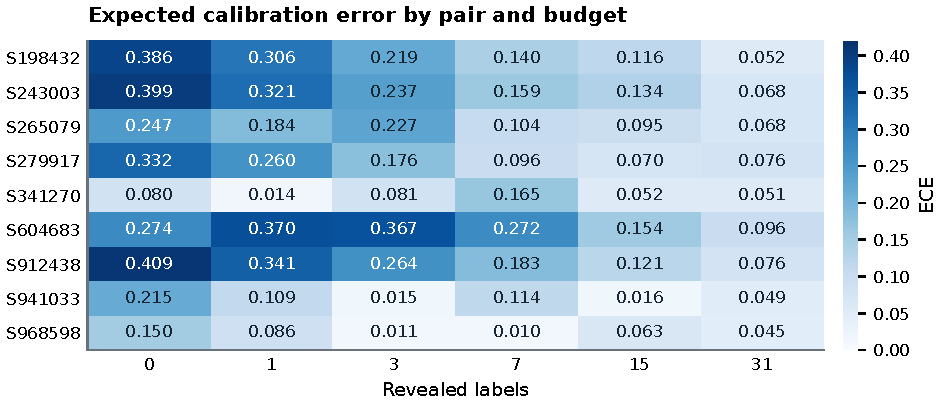
\includegraphics[width=.95\linewidth]{figures/ece_heatmap.pdf}
\caption{The complete ECE table as a heatmap. Darker cells indicate larger calibration error. A common color scale preserves comparisons across pairs and budgets.}
\end{figure}

\paragraph{Reconstruction tolerance.}
All analysis uses the supplied rounded values. Reconstructed pair ALCs differ from displayed pair summaries by at most $6\times10^{-7}$; the corresponding ECE discrepancy is at most $5\times10^{-7}$. Such differences are compatible with separately rounded inputs and summaries. The nine displayed ALC entries average exactly to the shown score of 0.160822.
